%\documentclass[5p,times]{elsarticle}
\documentclass[11pt,review,times]{elsarticle}

%%%%%%%%%%%%%%%%%%%%%%%%%%%%%%%%%%%%%%%%%%%%%%%%%%%%%%%%%%%%%%%%%
%	Loading packages
%%%%%%%%%%%%%%%%%%%%%%%%%%%%%%%%%%%%%%%%%%%%%%%%%%%%%%%%%%%%%%%%%
\usepackage[english]{babel}
\usepackage[utf8]{inputenc}
\usepackage[T1]{fontenc}
\usepackage{graphicx}
\usepackage{amsfonts}
\usepackage{placeins} % For /Floatbarrier
\usepackage{array,booktabs}
\usepackage{url} % For better linebreaks of URLs
\usepackage{float}
\usepackage{siunitx}
\usepackage{caption}
\usepackage{subcaption}
\usepackage{upgreek}
\usepackage[inline]{enumitem}
%\usepackage{mathrsfs}
%\usepackage{wasysym}
\usepackage{todonotes}


% Packages for tikz
\usepackage{tikz}
\usepackage{pgf}
\usepackage{pgfplotstable}
	\pgfplotstableset{col sep=comma} % call once in your preamble if all your tables use commas as column separator
	\pgfplotstableset{search path={datafiles}} % Put .csv files in /datafiles or the root folder
\usetikzlibrary{3d}
\usetikzlibrary{calc}
\usetikzlibrary{decorations.pathmorphing} % Pour obtenir des lignes de coupes aléatoires
\usetikzlibrary{arrows}
\usetikzlibrary{arrows.meta,shapes,positioning,shadows,trees,decorations.pathmorphing}
%\usetikzlibrary{external}
%\tikzexternalize[prefix=TikzPictures/]

\biboptions{sort&compress}

\newcolumntype{M}[1]{>{\centering\arraybackslash}m{#1}} % Define a column style "M" (verticaly centered by m) and horizontaly

% Hyperref and parameters of PDF
\usepackage[hidelinks]{hyperref}
\hypersetup{
	pdftitle = {Resistive welding of thermoplastic composites with a nanocomposite heating element},
    pdfauthor = {David Brassard, Martine Dubé, Jason R Tavares},
	pdfkeywords={carbon nanotube, thermal conductivity, polymer, nanocomposite, heating element, Joule heating, electrical conductivity, Finite element analysis, composite, thermoplastic},
	pdfsubject={Resistive welding of thermoplastic composites with a nanocomposite heating element}
}

\graphicspath{{Figures/}}	% Root directory of the pictures 

%%%%%%%%%%%%%%%%%%%%%%%%%%%%%%%%%%%%%%%%%%%%%%%%%%%%%%%%%%%%%%%%%
%	Main document
%%%%%%%%%%%%%%%%%%%%%%%%%%%%%%%%%%%%%%%%%%%%%%%%%%%%%%%%%%%%%%%%%
\begin{document}
\hyphenation{COMSOL na-no-com-po-si-te na-no-com-po-si-tes}


\title{Resistive welding of thermoplastic composites with a nanocomposite heating element}
\journal{TBD}

\author[polymtl,crepec]{David~Brassard}
\ead{david.brassard@polymtl.com}
\author[ets,crepec]{Martine~Dubé}
\ead{martine.dube@etsmtl.ca}
\author[polymtl,crepec]{Jason~R.~Tavares\corref{cor1}}
\ead{jason.tavares@polymtl.ca}

\cortext[cor1]{Corresponding author}

\address[polymtl]{Department of Chemical Engineering, Polytechnique Montréal, P.O. Box 6079 Station Centre-Ville, Montréal, QC, H3C 3A7, Canada}
\address[ets]{Department of Mechanical Engineering, École de technologie supérieure, 1100 Notre-Dame Street West, Montréal, Québec, Canada, H3C 1K3}
\address[crepec]{Research Center for High Performance Polymer and Composite Systems (CREPEC), Polytechnique Montréal, P.O. Box 6079 Station Centre-Ville, Montréal, QC, H3C 3A7, Canada}

\begin{abstract}
\todo[inline]{Write the abstract}
\end{abstract}

\begin{keyword}

\end{keyword}

\maketitle


%%%%%%%%%%%%%%%%%%%%%%%%%%%%%%%%%%%%%%%%%%%%%%%%%%%%%%%%%%%%%%%%%
							\section{Introduction}
%%%%%%%%%%%%%%%%%%%%%%%%%%%%%%%%%%%%%%%%%%%%%%%%%%%%%%%%%%%%%%%%%

The weight of structural elements has a strong impact on the efficiency and cost of transportation technologies. 
In the field of road transports car and truck makers are looking for new weight saving technologies \cite{FordMotorLLC2018} while life cycle analysis are confirming the gains from these transitions \cite{Cecchel2018,Meng2017}. 
Environmental regulations and costs are pushing the field of aeronautic toward carbon composite structures in planes \cite{Williams2003,Timmis2015}. 
Meanwhile, our increasing reliance on space technologies also drives aerospace toward composite materials to reduce the price to send cargo to orbit. 
More and more, fibre-reinforced plastics (FRP) are being used to produce lightweight structural elements. 

Thermoset composites are dominating the market for high performance FRP but thermoplastic composites are seeing an upward trend \cite{CompositeWorldSloan2018}. 
Demand for thermoplastic composites is driven by their higher impact resistance, increased production rate, superior recyclability and higher environmental resistance \cite{cogswell1992}. 
A distinct advantage of thermoplastics over thermoset is their ability to consolidate multiple components together via welding instead of using glue or mechanical fasteners. 

Resistance welding is a well established process to join thermoplastic composites. 
It is considered as a cost and weight effective solution. 
Initial developments involved the use of carbon fibre as heating elements \cite{houghton1984bonding,Eveno1988}.
Further development refined the process by optimizing the operational parameters \cite{Ageorges2000a}. 
Nevertheless, weld uniformity and electrical connections with the fibres was problematic and caused scaling issues \cite{McKnight1997}. 
To solve these issues, researchers looked for alternative heating elements.

Stainless steel meshes were found to increase the reliability of the process \cite{Hou1999a}. 
Effects of parameters such as the electrode distance and their geometry or the pattern of the electrical voltage applied were studied \cite{Dube2007}. 
Meanwhile, due to the importance of border effects, it was demonstrated that simple 2D simulations are not sufficient to model the process and full 3D simulations are required in order to optimize processing parameters  \cite{Talbot2013}. 
Other effects such as pressure on the weld and moisture content in the laminates also needs to be considered to obtain good welds \cite{Shi2014}.
Finally, the transition from a single step weld to continuous welding was devised and requires careful control of the whole process \cite{Shi2015a}. 

Common failure modes in single lap shear (SLS) tests for samples welded with stainless steel heating element are interfacial failure between the mesh and the polymer and tearing of the mesh for samples with suboptimal welding conditions and intralaminar failure accompanied by mesh tearing under good welding conditions \cite{Shi2014}. 
The peel stress is an important factor for crack propagation in SLS tests and, in that loading case, the metal mesh is solicitated in its \textit{z-axis} direction where it can't contribute \cite{Dube2008b}. 
This is also highlighted by the fact that an increase in open area of the mesh, to a certain extent, improved the SLS results \cite{Dube2012a}.

Traditional resistance welding with stainless steel heating elements is a well established process but we believe that it is interesting to keep investigating for alternative heating elements. 
Also, there is a need in the market for alternative welding process to match varied applications requirements \cite{CompositeWorldSloan2018}. 
With that in mind, we propose to look at conductive polymer nanocomposites as potential candidates to complement current stainless steel mesh welding technologies. 

Conductive nanocomposites comes from the combination of a polymer matrix and conductive nanoparticles. 
These conductive nanoparticles could be composed of metal or carbon. 
They can take shapes ranging from platelets, spheres or tubes and their size goes from the micrometre scale down to nanometre sized particles. 
Copper or silver nanowires \cite{Gelves2008a, Al-Saleh2011, Li2015a, Riviere2016}, carbon black \cite{Jin2013, MohdRadzuan2017}, graphene \cite{Jiang2012a, Hu2014a} and carbon nanotubes \cite{Diez-Pascual2011,Huegun2013,Kazakova2014,Jia2015} are a few of the commonly used particles. 
The electrical properties of the nanocomposites are dependant, among others, on the nature of the particles, their fraction, the mixing method and surface treatments. 
Even within the same kind of particles, variations in the manufacturing process can produce completely different results \cite{Bauhofer2009}. 
Thus the properties of nanocomposites need to be tailored for their applications to make use of their potential. 

Traditional metallic heating elements such as nichrome, or stainless steel in the case of resistive welding, relies on their relatively higher electrical resistance to produce heat through Joule effect. 
Although the electrical conductivity of conductive nanocomposites is much lower than usual values for conductors, they are able to generate controllable, sustained and repeatable localized heating \cite{Pyo2016}. 
In traditional resistance welding, polyetherimide (PEI) is commonly used to provide a resin rich region to prevent current leakage through the composite. 
Its miscibility with poly(ether ether ketone) (PEEK) \cite{Crevecoeur1991} also helps to obtain good mechanical performances.
By using the same polymer for the matrix of the nanocomposite, we hypothesize that we could take advantage of that miscibility and obtain a nanocomposite heating element appropriate for resistance welding of high performance thermoplastic composite. 
This novel heating element would be almost entirely miscible within the matrix of the composite and would not leave foreign objects in the weld. 


%%%%%%%%%%%%%%%%%%%%%%%%%%%%%%%%%%%%%%%%%%%%%%%%%%%%%%%%%%%%%%%%%
							\section{Methodology}
%%%%%%%%%%%%%%%%%%%%%%%%%%%%%%%%%%%%%%%%%%%%%%%%%%%%%%%%%%%%%%%%%

%%%%%%%%%%%%%%%%%%%%%%%%%%%%%%%%%%%%%%%%%%%%%%%%%%%%%%%%%%%%%%
\subsection{Simulations}
%%%%%%%%%%%%%%%%%%%%%%%%%%%%%%%%%%%%%%%%%%%%%%%%%%%%%%%%%%%%%%

A first method to explore the process was to model the heating of nanocomposites with COMSOL Mul\-ti\-phy\-sics\-\textregistered.  
A set of three continuum micromechanic models observed different contact topologies and their relative contribution to the heating phenomena within a nanocomposite. 
The goal of these simulations was to ascertain that the polymer is not thermally degraded by localized heat concentration due to the lower thermal conductivity of the polymer. 
Representative elementary volume (REV) were used in these models (Fig. \ref{fig:geometry}). 
A mass fraction of 1\% MWCNTs was taken as reference. 

\begin{figure}[htb]
	\center
	\begin{subfigure}{40mm}
		\center
		\captionsetup{width=35mm}
		\resizebox{35mm}{!}{
		%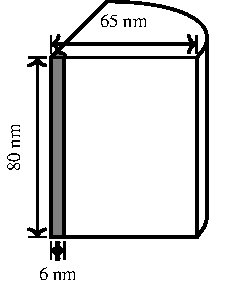
\includegraphics[width=35mm]{geometry_axisymmetric}
		%\tikzsetnextfilename{geometry_axisymmetric}
		%\shorthandoff{:!}

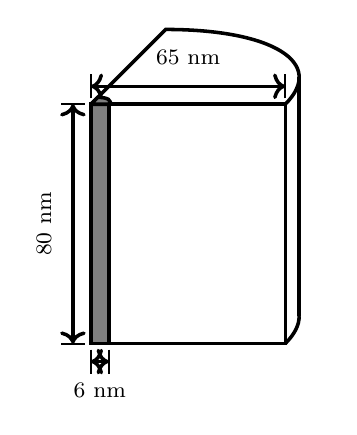
\begin{tikzpicture}[scale=0.038]

%%%%%%%%%%%%%%%%%%%%%%
%%%	 Def géométrie  %%%
%%%%%%%%%%%%%%%%%%%%%%

\def \rayonun{6}
\def \rayondeux{65}
\def \vspace{2}
\def \lignecote{8}
\def \hauteur{80}
\def \anglearc{111.5}

%%%%%%%%%%%%%%%%%%%%%%
%%%	   Def style    %%%
%%%%%%%%%%%%%%%%%%%%%%

\def \heavy{0.045cm}
\def \light{0.025cm}

%%%%%%%%%%%%%%%%%%%%%%
%%%	    Calculs     %%%
%%%%%%%%%%%%%%%%%%%%%%

\pgfmathsetmacro{\sinangle}{sin(\anglearc)}
\pgfmathsetmacro{\cosangle}{cos(\anglearc)}

%%%%%%%%%%%%%%%%%%%%%%
%%%	    Dessin      %%%
%%%%%%%%%%%%%%%%%%%%%%

\draw[line width=\heavy] (\rayonun,0) rectangle (\rayondeux,\hauteur);
\draw[line width=\heavy, fill=gray] (0,0) rectangle (\rayonun,\hauteur);
%\draw[line width=\heavy] \draw (0,0,0) arc (0:45:1) ;

% On se positionne sur un plan à une hauteur de 80 (\hauteur)
\begin{scope}[canvas is zx plane at y=\hauteur]
	% On dessine le quart de cercle extérieur
	\draw[line width=\heavy] (0,\rayondeux) arc (90:180:\rayondeux) -- (0,0);
	% On dessine le quart de cercle du nanotube
	\draw[line width=\heavy, fill=gray] (0,0) -- (0,\rayonun) arc (90:180:\rayonun) -- (0,0);
\end{scope}

% On se positionne sur un plan à une hauteur de 0
\begin{scope}[canvas is zx plane at y=0]
	% On trace le cercle jusqu'à l'angle \anglearc trouvé itérativement
	\draw[line width=\heavy] (0,\rayondeux) arc (90:\anglearc:\rayondeux);
\end{scope}

% Ligne du côté du cylindre
\draw[line width=\heavy] (\sinangle*\rayondeux,0,\cosangle*\rayondeux) -- +(0,\hauteur,0);

%%%%%%%%%%%%%%%%%%%%%%
%%%	    Cotation    %%%
%%%%%%%%%%%%%%%%%%%%%%

% On dessine la ligne de cote pour la nanotube
\draw[line width=\light] (0,-\vspace) -- + (0,-\lignecote);
\draw[line width=\light] (\rayonun,-\vspace) -- + (0,-\lignecote);
\draw[<->,line width=\heavy] (0,-\vspace-0.5*\lignecote) -- + (\rayonun,0);

\node[anchor=north] (A) at (0.5*\rayonun , -\vspace-\lignecote) {\footnotesize \rayonun \ nm};

% On dessine la ligne de cote pour la hauteur
\draw[line width=\light] (-\vspace,0) -- + (-\lignecote,0);
\draw[line width=\light] (-\vspace,\hauteur) -- + (-\lignecote,0);
\draw[<->,line width=\heavy] (-\vspace-0.5*\lignecote,0) -- + (0,\hauteur);

\node[anchor=south, rotate=90] (A) at (-\vspace-\lignecote,0.5*\hauteur ) {\footnotesize \hauteur \ nm};

% On dessine la ligne de cote pour le diamètre du modèle
\draw[line width=\light] (0,\hauteur+\vspace) -- + (0,\lignecote);
\draw[line width=\light] (\rayondeux,\hauteur+\vspace) -- + (0,\lignecote);
\draw[<->,line width=\heavy] (0,\hauteur+\vspace+0.5*\lignecote) -- + (\rayondeux,0);

\node[anchor=south] (A) at (0.5*\rayondeux , \hauteur+\vspace+\lignecote) {\footnotesize \rayondeux \ nm};

%%%%%%%%%%%%%%%%%%%%%%%%%%%%%%%%%%%%%%%%%

\end{tikzpicture}

%\shorthandon{:!}
		}
		\caption{Quarter section of the geometry of the first FEM simulating the Joule heating within a MWCNT}
		\label{fig:geometry_axisymmetric}
	\end{subfigure}%
	\begin{subfigure}{55mm}
		\center
		\captionsetup{width=50mm}
		\resizebox{65mm}{!}{
		%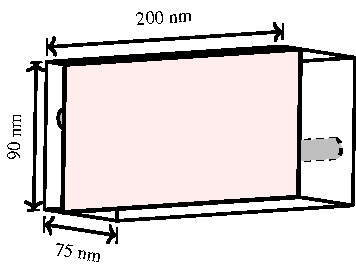
\includegraphics[width=50mm]{geometry_3D}
		%\tikzsetnextfilename{geometry_3D}
		%\shorthandoff{:!}

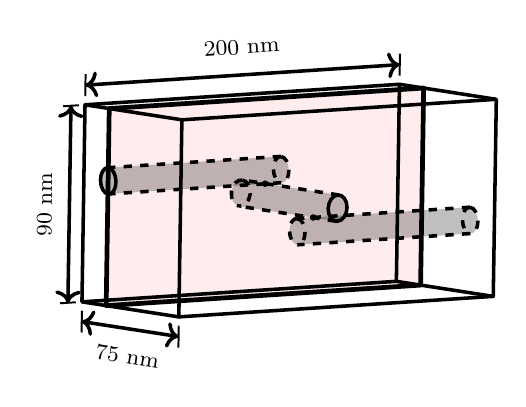
\begin{tikzpicture}[scale=0.02,
								x  = {(0.99788,0.065079)},
                    		y  = {(0.021693,1.38835)},
                    		z  = {(-0.824336,0.130158)},]

%%%%%%%%%%%%%%%%%%%%%%
%%%	 Def géométrie  %%%
%%%%%%%%%%%%%%%%%%%%%%

\def \dia{6} %La variable dia contient en fait le rayon des tubes au lieu du diamètre
\def \epaisseur{75}
\def \hauteur{90}
\def \longueur{200}

\def \angle{88.0}

\def \vspace{4}
\def \lignecote{10}
\def \anglearc{111.5}

\def \colplan{red!7}
\def \coltube{gray!50}

\def \dotsize{60pt}

\coordinate (A) at (0,0,0);
\coordinate (B) at (0,0,\epaisseur);
\coordinate (C) at (0,\hauteur,\epaisseur);
\coordinate (D) at (0,\hauteur,0);
\coordinate (E) at (-\longueur,0,0);
\coordinate (F) at (-\longueur,0,\epaisseur);
\coordinate (G) at (-\longueur,\hauteur,\epaisseur);
\coordinate (H) at (-\longueur,\hauteur,0);

\coordinate (W) at (0,0,0.75*\epaisseur);
\coordinate (X) at (0,\hauteur,0.75*\epaisseur);
\coordinate (Y) at (-\longueur,\hauteur,0.75*\epaisseur);
\coordinate (Z) at (-\longueur,0,0.75*\epaisseur);


%%%%%%%%%%%%%%%%%%%%%%
%%%	   Def style    %%%
%%%%%%%%%%%%%%%%%%%%%%

\def \heavy{0.045cm}
\def \light{0.025cm}
\def \reallyheavy{0.06cm}

%Modification du monde de transparence pour mélanger les couleurs superposées
\begin{scope}[blend mode=multiply]

%%%%%%%%%%%%%%%%%%%%%%
%%%	    Calculs     %%%
%%%%%%%%%%%%%%%%%%%%%%

\pgfmathsetmacro{\sinangle}{sin(\anglearc)}
\pgfmathsetmacro{\cosangle}{cos(\anglearc)}

\pgfmathsetmacro{\sinangledeux}{sin(\angle)}
\pgfmathsetmacro{\cosangledeux}{cos(\angle)}

%%%%%%%%%%%%%%%%%%%%%%
%%%	 Dessin du cube %%%
%%%%%%%%%%%%%%%%%%%%%%

\draw[line width=\heavy, line join=round] (A) -- (B) -- (C) --(D) -- cycle;
\draw[line width=\heavy, line join=round] (E) -- (F) -- (G) --(H) -- cycle;
\draw[line width=\heavy, line join=round] (D) -- (H);
\draw[line width=\heavy, line join=round] (G) -- (C);
\draw[line width=\heavy, line join=round] (A) -- (E);
\draw[line width=\heavy, line join=round] (F) -- (B);


%%%%%%%%%%%%%%%%%%%%%%%%%%%%%%%%%%%%
%%% Dessin du nanotube du centre %%%
%%%%%%%%%%%%%%%%%%%%%%%%%%%%%%%%%%%%

%Trouver les distances projetées en x et y pour un vecteur unitaire pour chaque axe
\path (1,0,0);
\pgfgetlastxy{\cylxx}{\cylxy}
\path (0,1,0);
\pgfgetlastxy{\cylyx}{\cylyy}
\path (0,0,1);
\pgfgetlastxy{\cylzx}{\cylzy}

%Calculs
\pgfmathsetmacro{\cylt}{(\cylzy * \cylyx - \cylzx * \cylyy)/ (\cylzy * \cylxx - \cylzx * \cylxy)}
\pgfmathsetmacro{\ang}{atan(\cylt)}
\pgfmathsetmacro{\ct}{1/sqrt(1 + (\cylt)^2)}
\pgfmathsetmacro{\st}{\cylt * \ct}

%\node[anchor=north] (A) at (0,-30,0) {\large xx \cylxx};
%\node[anchor=north] (A) at (0,-40,0) {\large xy \cylxy};
%\node[anchor=north] (A) at (0,-50,0) {\large yx \cylyx};
%\node[anchor=north] (A) at (0,-60,0) {\large yy \cylyy};
%\node[anchor=north] (A) at (0,-70,0) {\large zx \cylzx};
%\node[anchor=north] (A) at (0,-80,0) {\large zy \cylzy};
%\node[anchor=north] (A) at (0,-90,0) {\large \cylt};
%\node[anchor=north] (A) at (0,-100,0) {\large \ang};
%\node[anchor=north] (A) at (0,-110,0) {\large \ct};
%\node[anchor=north] (A) at (0,-120,0) {\large \st};

%\draw[line width=0.45, line join=round] (A) -- (H);

%Surface extérieure du cylindre
\fill[\coltube] (-0.5*\longueur+\dia*\ct,0.5*\hauteur+\dia*\st,\epaisseur) -> ++(0,0,-\epaisseur) arc[start angle=\ang,delta angle=180,radius=\dia] -- ++(0,0,\epaisseur) arc[start angle=\ang+180,delta angle=-180,radius=\dia];

%Lignes des côtés
\begin{scope}[every path/.style={line width=\heavy}]

	%Cercle du devant
	\draw[fill=\coltube] (-0.5*\longueur,0.5*\hauteur,0) circle[radius=\dia];

	%Ligne des côtés
	\draw[dashed] (-0.5*\longueur+\dia*\ct,0.5*\hauteur+\dia*\st,0) -- ++(0,0,\epaisseur);
	\draw[dashed] (-0.5*\longueur-\dia*\ct,0.5*\hauteur-\dia*\st,0) -- ++(0,0,\epaisseur);

	%Cercle arrière
	\draw[dashed] (-0.5*\longueur+\dia*\ct,0.5*\hauteur+\dia*\st,\epaisseur) arc[start angle=\ang,delta angle=180,radius=\dia];
	\draw[dashed] (-0.5*\longueur+\dia*\ct,0.5*\hauteur+\dia*\st,\epaisseur) arc[start angle=\ang,delta angle=-180,radius=\dia];
	
\end{scope}

%\draw (-0.5*\longueur,.5*\hauteur,0) -- (-0.5*\longueur,.5*\hauteur,\epaisseur);

%%%%%%%%%%%%%%%%%%%%%%%%%%%%%%%%%%%%
%%% Dessin du nanotube de droite %%%
%%%%%%%%%%%%%%%%%%%%%%%%%%%%%%%%%%%%

\begin{scope}[canvas is zy plane at x=0]
	\draw[line width=\heavy, dashed] (0.25*\epaisseur,0.5*\hauteur-2*\dia) ++(\angle:\dia) arc[start angle=\angle,delta angle=-180,radius=\dia];
	\draw[line width=\heavy, dashed, fill=\coltube] (0.25*\epaisseur,0.5*\hauteur-2*\dia) ++(\angle:\dia) arc[start angle=\angle,delta angle=180,radius=\dia];
\end{scope}


\begin{scope}[canvas is zy plane at x=-0.55*\longueur]
	\draw[line width=\heavy, dashed, fill=\coltube] (0.25*\epaisseur,0.5*\hauteur-2*\dia) ++(\angle:\dia) arc[start angle=\angle,delta angle=-180,radius=\dia];
	\draw[line width=\heavy, dashed] (0.25*\epaisseur,0.5*\hauteur-2*\dia) ++(\angle:\dia) arc[start angle=\angle,delta angle=180,radius=\dia];
\end{scope}


\draw[line width=\heavy, dashed] (0,0.5*\hauteur-2*\dia+\dia*\sinangledeux,0.25*\epaisseur+\dia*\cosangledeux) -- ++(-0.55*\longueur,0,0);	

\draw[line width=\heavy, dashed] (0,0.5*\hauteur-2*\dia-\dia*\sinangledeux,0.25*\epaisseur-\dia*\cosangledeux) -- ++(-0.55*\longueur,0,0);	

\fill[\coltube] (0,0.5*\hauteur-2*\dia+\dia*\sinangledeux,0.25*\epaisseur+\dia*\cosangledeux) -- ++(-0.55*\longueur,0,0) -- ++(0,-2*\dia*\sinangledeux,-2*\dia*\cosangledeux)-- ++(0.55*\longueur,0,0) -- cycle;

%\draw (0,0.5*\hauteur-\dia,\epaisseur*0.25) -- ++(-0.55*\longueur,0,0);


%%%%%%%%%%%%%%%%%%%%%%%%%%%%%%%%%%%%
%%% Dessin du nanotube de gauche %%%
%%%%%%%%%%%%%%%%%%%%%%%%%%%%%%%%%%%%


\begin{scope}[canvas is zy plane at x=-\longueur]
	\draw[line width=\heavy, fill=\coltube] (0.75*\epaisseur,0.5*\hauteur+2*\dia) ++(\angle:\dia) arc[start angle=\angle,delta angle=-180,radius=\dia];
	\draw[line width=\heavy] (0.75*\epaisseur,0.5*\hauteur+2*\dia) ++(\angle:\dia) arc[start angle=\angle,delta angle=180,radius=\dia];
\end{scope}

\begin{scope}[canvas is zy plane at x=-0.45*\longueur]
	\draw[line width=\heavy, dashed] (0.75*\epaisseur,0.5*\hauteur+2*\dia) ++(\angle:\dia) arc[start angle=\angle,delta angle=-180,radius=\dia];
	\draw[line width=\heavy, dashed, fill=\coltube] (0.75*\epaisseur,0.5*\hauteur+2*\dia) ++(\angle:\dia) arc[start angle=\angle,delta angle=180,radius=\dia];
\end{scope}

\draw[line width=\heavy, dashed] (-0.45*\longueur,0.5*\hauteur+2*\dia+\dia*\sinangledeux,0.75*\epaisseur+\dia*\cosangledeux) -- ++(-0.55*\longueur,0,0);	

\draw[line width=\heavy, dashed] (-0.45*\longueur,0.5*\hauteur+2*\dia-\dia*\sinangledeux,0.75*\epaisseur-\dia*\cosangledeux) -- ++(-0.55*\longueur,0,0);	

\fill[\coltube] (-0.45*\longueur,0.5*\hauteur+2*\dia+\dia*\sinangledeux,0.75*\epaisseur+\dia*\cosangledeux) -- ++(-0.55*\longueur,0,0) -- ++(0,-2*\dia*\sinangledeux,-2*\dia*\cosangledeux)-- ++(0.55*\longueur,0,0) -- cycle;

%%%%%%%%%%%%%%%%%%%%%%%%%%%%%%%%%%%%
%%% Dessin des points de contact %%%
%%%%%%%%%%%%%%%%%%%%%%%%%%%%%%%%%%%%

\fill [black] (-0.5*\longueur,0.5*\hauteur-\dia,0.25*\epaisseur) circle (\dotsize);
\fill [black] (-0.5*\longueur,0.5*\hauteur+\dia,0.75*\epaisseur) circle (\dotsize);

%%%%%%%%%%%%%%%%%%%%%%%%%%%%%%%%%%%%
%%% Dessin du plan de decoupe    %%%
%%%%%%%%%%%%%%%%%%%%%%%%%%%%%%%%%%%%

\draw[line width=\reallyheavy, line join=round, fill=\colplan] (W) -- (X) -- (Y) --(Z) -- cycle;

%%%%%%%%%%%%%%%%%%%%%%
%%%	    Cotation    %%%
%%%%%%%%%%%%%%%%%%%%%%

%Calcul des angles de rotation pour les cotes
\pgfmathsetmacro{\rotx}{ atan( \cylxy / \cylxx) }
\pgfmathsetmacro{\roty}{ atan( \cylyx / \cylyy) }
\pgfmathsetmacro{\rotz}{ atan( \cylzy / \cylzx) }

% On dessine la ligne de cote pour la longueur
\draw[line width=\light] (-\longueur,\vspace+\hauteur,\epaisseur) -- + (0,\lignecote,0);
\draw[line width=\light] (0,\vspace+\hauteur,\epaisseur) -- + (0,\lignecote,0);
\draw[<->,line width=\heavy] (-\longueur,+\vspace+\hauteur+0.5*\lignecote,\epaisseur) -- + (\longueur,0,0);

\node[anchor=south, rotate=\rotx] (C) at (-0.5*\longueur,\hauteur+\vspace+\lignecote,\epaisseur ) {\footnotesize \longueur \ nm};

% On dessine la ligne de cote pour la hauteur
\draw[line width=\light] (-\longueur-\vspace,0,\epaisseur) -- + (-\lignecote,0,0);
\draw[line width=\light] (-\longueur-\vspace,\hauteur,\epaisseur) -- + (-\lignecote,0);
\draw[<->,line width=\heavy] (-\longueur-\vspace-0.5*\lignecote,0,\epaisseur) -- + (0,\hauteur);

\node[anchor=south, rotate=90-\roty] (C) at (-\longueur-\vspace-\lignecote,0.5*\hauteur,\epaisseur ) {\footnotesize \hauteur \ nm};

% On dessine la ligne de cote pour l'épaisseur
\draw[line width=\light] (-\longueur,-\vspace,\epaisseur) -- + (0,-\lignecote,0);
\draw[line width=\light] (-\longueur,-\vspace,0) -- + (0,-\lignecote,0);
\draw[<->,line width=\heavy] (-\longueur,-\vspace-0.5*\lignecote,\epaisseur) -- + (0,0,-\epaisseur);

\node[anchor=north, rotate=\rotz] (C) at (-\longueur,-\vspace-\lignecote,0.5*\epaisseur ) {\footnotesize \epaisseur \ nm};

\end{scope}

\end{tikzpicture}

%\shorthandon{:!}
		}
		\caption{Geometry of the second FEM evaluating the effect of charge concentration at contact point}
		\label{fig:geometry_3D}
	\end{subfigure}
	\begin{subfigure}{40mm}
		\center
		\captionsetup{width=40mm}
		\resizebox{35mm}{!}{
		%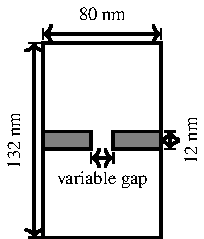
\includegraphics[width=40mm]{geometry_gap}
		%\tikzsetnextfilename{geometry_gap}
		%\shorthandoff{:!}

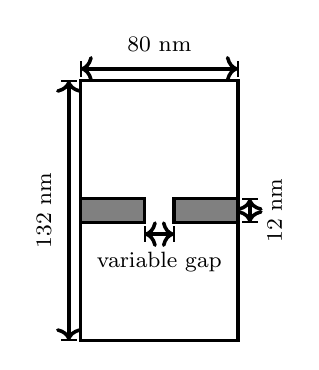
\begin{tikzpicture}[scale=0.025]

%%%%%%%%%%%%%%%%%%%%%%
%%%	 Def géométrie  %%%
%%%%%%%%%%%%%%%%%%%%%%

\def \diacnt{12}
\def \longueur{80}
\def \vspace{2}
\def \lignecote{8}
\def \hauteur{132}
\def \anglearc{111.5}
\def \gap{15}

%%%%%%%%%%%%%%%%%%%%%%
%%%	   Def style    %%%
%%%%%%%%%%%%%%%%%%%%%%

\def \heavy{0.045cm}
\def \light{0.025cm}

%%%%%%%%%%%%%%%%%%%%%%
%%%	    Calculs     %%%
%%%%%%%%%%%%%%%%%%%%%%

\pgfmathsetmacro{\sinangle}{sin(\anglearc)}
\pgfmathsetmacro{\cosangle}{cos(\anglearc)}

%%%%%%%%%%%%%%%%%%%%%%
%%%	    Dessin      %%%
%%%%%%%%%%%%%%%%%%%%%%

\draw[line width=\heavy] (0,0) rectangle (\longueur,\hauteur);
\draw[line width=\heavy, fill=gray] (0,0.5*\hauteur-0.5*\diacnt) rectangle (0.5*\longueur-0.5*\gap,0.5*\hauteur+0.5*\diacnt);
\draw[line width=\heavy, fill=gray] (0.5*\longueur+0.5*\gap,0.5*\hauteur-0.5*\diacnt) rectangle (\longueur,0.5*\hauteur+0.5*\diacnt);


%%%%%%%%%%%%%%%%%%%%%%
%%%	    Cotation    %%%
%%%%%%%%%%%%%%%%%%%%%%

% On dessine la ligne de cote pour l'espace entre les nanotubes
\draw[line width=\light] (0.5*\longueur-0.5*\gap,-\vspace+0.5*\hauteur-0.5*\diacnt) -- + (0,-\lignecote);
\draw[line width=\light] (0.5*\longueur+0.5*\gap,-\vspace+0.5*\hauteur-0.5*\diacnt) -- + (0,-\lignecote);
\draw[<->,line width=\heavy] (0.5*\longueur-0.5*\gap,-\vspace-0.5*\lignecote+0.5*\hauteur-0.5*\diacnt) -- + (\gap,0);

\node[anchor=north] (A) at (0.5*\longueur , -\vspace-\lignecote+0.5*\hauteur-0.5*\diacnt) {\footnotesize variable gap};

% On dessine la ligne de cote pour le diamètre des nanotubes
\draw[line width=\light] (\longueur+\vspace,0.5*\hauteur-0.5*\diacnt) -- + (\lignecote,0);
\draw[line width=\light] (\longueur+\vspace,0.5*\hauteur+0.5*\diacnt) -- + (\lignecote,0);
\draw[<->,line width=\heavy] (\longueur+\vspace+0.5*\lignecote,0.5*\hauteur-0.5*\diacnt) -- + (0,\diacnt);

\node[anchor=north, rotate=90] (B) at (\longueur+\vspace+\lignecote,0.5*\hauteur ) {\footnotesize \diacnt \ nm};

% On dessine la ligne de cote pour la hauteur
\draw[line width=\light] (-\vspace,0) -- + (-\lignecote,0);
\draw[line width=\light] (-\vspace,\hauteur) -- + (-\lignecote,0);
\draw[<->,line width=\heavy] (-\vspace-0.5*\lignecote,0) -- + (0,\hauteur);

\node[anchor=south, rotate=90] (C) at (-\vspace-\lignecote,0.5*\hauteur ) {\footnotesize \hauteur \ nm};

% On dessine la ligne de cote pour le diamètre du modèle
\draw[line width=\light] (0,\hauteur+\vspace) -- + (0,\lignecote);
\draw[line width=\light] (\longueur,\hauteur+\vspace) -- + (0,\lignecote);
\draw[<->,line width=\heavy] (0,\hauteur+\vspace+0.5*\lignecote) -- + (\longueur,0);

\node[anchor=south] (D) at (0.5*\longueur , \hauteur+\vspace+\lignecote) {\footnotesize \longueur \ nm};

%%%%%%%%%%%%%%%%%%%%%%%%%%%%%%%%%%%%%%%%%

\end{tikzpicture}

%\shorthandon{:!}
		}
		\caption{Geometry of the third FEM simulating Joule heating within the polymer matrix}
		\label{fig:geometry_gap}
	\end{subfigure} 
	\caption{Geometries of the representative elementary volume composed of MWCNT (dark region) and the insulating matrix (white region)}
	\label{fig:geometry}
\end{figure}

The goal of the first topology was to model simple conduction along the length of a single multiwalled carbon nanotube (MWCNT) and the resulting Joule heating. 
In this axisymmetric model (Fig. \ref{fig:geometry_axisymmetric}), the REV consisted of a cylindrical MWCNT (dark region) surrounded by the insulating matrix (white region). 
The top and bottom surfaces of the MWCNT acted as voltage source and ground, respectively, with the current flowing through the MWCNT. 
The diameter of the MWCNT was set to \SI{12}{\nano\metre} in agreement with the data obtained from our supplier. 

In the second topology, the flow of current has to transition through direct contact between adjacent nanotubes. 
The REV (Fig. \ref{fig:geometry_3D}) included three MWCNTs (dark region) that formed a percolated electrical path within the polymer matrix. 
The current from the voltage source must transfer through two contact point interfaces to reach the ground on the other side of the conductive network. 
The highlighted plane shows the area of interest for temperature monitoring. 
Joule heating from within the MWCNTs was also present in this model. 

For the third topology, the current was forced to flow through the polymer between two adjacent MWCNTs.
In this REV, a gap of variable length was introduced between the ends of two conductive MWCNTs (Fig. \ref{fig:geometry_gap}). 
This gap forced the flow of current to travel through the polymer.  

In each simulation, a constant DC electric field was applied for \SI{5}{\second} and the resulting temperature field was recorded. 
The value of the electric field was adjusted so as to get similar temperatures after \SI{5}{\second} in all three models. 
Volumetric and boundary electromagnetic heat sources were used to simulate Joule heating. 
Conductive heat transfer within solids (Fourier's law) is considered and the current is conserved within the elementary volume (conservation law). 
Electrical insulation and symmetric thermal boundary conditions were set for the edges of the polymer matrix that were not in contact with the MWCNT. 
Symmetric thermal boundary conditions were defined at both ends of the MWCNT. 
These boundary conditions were selected to simulate a REV far from the outer surfaces. 
Under these conditions, heat was generated within the three models but had no way to exit, causing the temperature to increase as energy kept accumulating.

The physical properties of PEEK were used for the polymer matrix alongside physical properties for MWCNT taken from the literature (Tab. \ref{tab:material_properties}). 

\begin{table}[htb]
\center
\resizebox{125mm}{!}{
\begin{tabular}{@{}lllrlrl@{}}
\toprule
Property    					&                   &        												& PEEK & 																		& MWCNT 					& \\ \midrule
Density						& $\rho$            & [\si{\kilo\gram\per\cubic\metre}]  			& 1300 & \cite{cogswell1992, Giants1994}							& 2000 					& \cite{Lehman2011} \\
Specific heat				& $C_p$             & [\si{\joule\per\kilo\gram\per\celsius}] 	& 1950 & \cite{cogswell1992}											& 600 						& \cite{Mizel99} \\
Thermal conductivity		& $k$               & [\si{\watt\per\metre\per\celsius}]  			& 0.25 & \cite{cogswell1992}											& 3000						& \cite{Mizel99,Berber2000} \\
Electrical conductivity	& $\sigma$          & [\si{\siemens\per\metre}]    					& $2 \times 10^{-14}$ & \cite{Giants1994,Bangarusampath2009}	& $8.3 \times 10^5$	& \cite{Ebbesen1996} \\
Relative permittivity		& $\upvarepsilon_r$ & [ \sep ]												& 3.1  &	\cite{victrexpeek, Giants1994}								& 12.5     				& \cite{Katsounaros2011} \\ \bottomrule
\end{tabular}}
\caption{Material properties}
\label{tab:material_properties}
\end{table}


%%%%%%%%%%%%%%%%%%%%%%%%%%%%%%%%%%%%%%%%%%%%%%%%%%%%%%%%%%%%%%
\subsection{Materials}
%%%%%%%%%%%%%%%%%%%%%%%%%%%%%%%%%%%%%%%%%%%%%%%%%%%%%%%%%%%%%%

\subsubsection{Polymers and nanocomposite}

The polymer materials were PEEK (CAS 29658-26-2) and PEI (CAS 61128-46-9) pellets ordered from Sigma Aldrich. 
PEEK pellets had an average molecular weight by mass ($M_w$) of \SI{20,8}{\kilo\gram\per\mol} and an average molecular mass by number ($M_n$) of \SI{10,3}{\kilo\gram\per\mol} and PEI pellets had a melt index of \SI{18}{\gram} per \SI{10}{\minute} at \SI{337}{\celsius} with a mass of \SI{6.6}{\kilogram}. 

The conductive nanoparticles consisted of dry powdered MWCNTs, produced by combustion chemical vapour deposition (CCVD), purchased from Raymor Industries. 
They had outer diameters in the range of 10 to \SI{20}{\nano\metre}, lengths from 1 to \SI{12}{\micro\metre} and purity of at least 99\%.

The nanocomposites were produced with a DSM Xplore 5 cc twin screw micro compounder. 
Polymer pellets were introduced along with the MWCNTs and internally mixed by the recirculation circuit. 
The resulting batches of extruded wires were cut into small pellets, mixed thoroughly and fed a second time to obtain uniform mixing. 
The PEI and PEEK nanocomposites were respectively processed at 340 and \SI{390}{\celsius}. 
Nanocomposite extruded from the micro compounder with a die diameter of 1 mm was used as is for the PEEK nanocomposite wire, with a 16\% mass fraction of MWCNTs. 
Flat PEI nanocomposite heating elements, with a 10\% mass fraction of MWCNTs, were produced by hot pressing films and cutting them to dimensions. 
The electrical conductivity of the PEI nanocomposite, at 5\%, 10\% and 15\% mass fraction of MWCNTs, was measured with the four-point probe technique. 

\subsubsection{Composite}

The composite adherents were produced by hot pressing PEEK/CF pre-preg sheets to form unidirectional composite panels. 
The laminate were heated at a temperature of \SI{390}{\celsius} and then consolidated with a pressure of \SI{2}{\mega\pascal} for \SI{30}{\minute} before cooling them, in agreement to the supplier's recommendations. 
The composite adherents were cut to dimensions, with an abrasive saw, according to ASTM D5868 - 01(2014). 

%%%%%%%%%%%%%%%%%%%%%%%%%%%%%%%%%%%%%%%%%%%%%%%%%%%%%%%%%%%%%%
\subsection{Small scale experiments}
%%%%%%%%%%%%%%%%%%%%%%%%%%%%%%%%%%%%%%%%%%%%%%%%%%%%%%%%%%%%%%

Prior to the welding tests, a simple small scale validation of the heating elements was devised. 
A \SI{1}{\milli\metre} PEEK wire approximately \SI{80}{\milli\metre} long was attached to an AC power source with adjustable voltage
Five different voltages (from 10 to \SI{50}{\volt}) were applied to the sample to obtain five different power levels. 
Tests were conducted under a fume hood.
The voltage and current were measured once the temperature in the wire reached steady state. 
The value of the electric field was obtained by dividing the voltage from the source by the length of the wire between the electrical connectors. 
A FLIR T420 infrared camera was used to record the surface temperature distribution. 

%%%%%%%%%%%%%%%%%%%%%%%%%%%%%%%%%%%%%%%%%%%%%%%%%%%%%%%%%%%%%%
\subsection{Welding experiments}
%%%%%%%%%%%%%%%%%%%%%%%%%%%%%%%%%%%%%%%%%%%%%%%%%%%%%%%%%%%%%%

The third stage is to demonstrate the capability of the nanocomposite heating element to serve as a viable alternative to stainless steel meshes for resistance welding of high performance thermoplastic composites. 
A computer controlled resistance welding jig was built to weld single lap shear test samples with an overlap of \SI{12.7}{\milli\metre} and a width of \SI{25.4}{\milli\metre}. 
Two machined copper electrodes were used to connect the power source to the nanocomposite heating element. 
Three pneumatic actuators applied constant pressure over the electrodes and the welded zone while the nanocomposite was kept between two composite adherents surrounded by Alumina-Silicate ceramic insulating blocks. 
Electrical power was supplied by a \SI{10}{\kilo\watt} programmable DC power source series XR from Magna-Power capable of delivering up to \SI{160}{\volt} and \SI{60}{\ampere}. 
The power source can be driven as a constant voltage source, constant current source or with custom power profiles. 
A modulation scheme was developed to allow the source to operate with a constant power output. 
In this mode, the source adjusts its output current based on the voltage applied and keep a constant power output disregarding variations in the resistance of the heating element. 

\missingfigure{Photo/CAD of the welding jig or an easier to read schematic?}

For the welding experiments, electrical parameters were set as to mimic conditions that are observed during traditional resistance welding of thermoplastic composites. 
The initial voltage setting for constant voltage operation was calculated based on a specific power of \SI{350}{\kilo\watt\per\square\metre} and the electrical resistance of the heating element. 

Prior to welding, the surfaces of the adherents and the nanocomposite were thoroughly cleaned with acetone to remove any traces of residue or release agent. 
PEI nanocomposite heating elements, with a thickness of \SI{0.5}{\milli\metre} and a width of \SI{12.7}{\milli\metre}, were installed between the composite adherents. 
Tabs on both ends were left to connect the electrodes, they were laying flat on ceramic insulator blocks while the pneumatic actuators pushed the copper electrodes against them. 
A contact pressure of \SI{2.4}{\mega\pascal} was applied by the electrodes over a square area with \SI{12.7}{\milli\metre} sides. 
Over the weld, a third actuator applied a constant pressure of \SI{1}{\mega\pascal} during the whole welding process. 
It was previously demonstrated, for traditional resistance welding, that a \SI{1}{\mega\pascal} pressure can produce good welds \cite{Ageorges2000a, Dube2007, Shi2014}.
Type K thermocouples, located on the ceramic above the welded zone, monitored the temperature during the welding process (Fig. \ref{fig:location_thermocouple}).
Thermocouples could not be installed directly on the nanocomposite films as their presence altered the heat transfer mechanisms within the weld. 
The first thermocouple was located slightly off center at \SI{14}{\milli\metre} from the side of the adherent at the centerline of the overlap. 
The second thermocouple was located on the centerline but \SI{2.5}{\milli\metre} away from the side of the adherent.  

\begin{figure}
		\center
		\captionsetup{width=60mm}
		\resizebox{60mm}{!}{
		%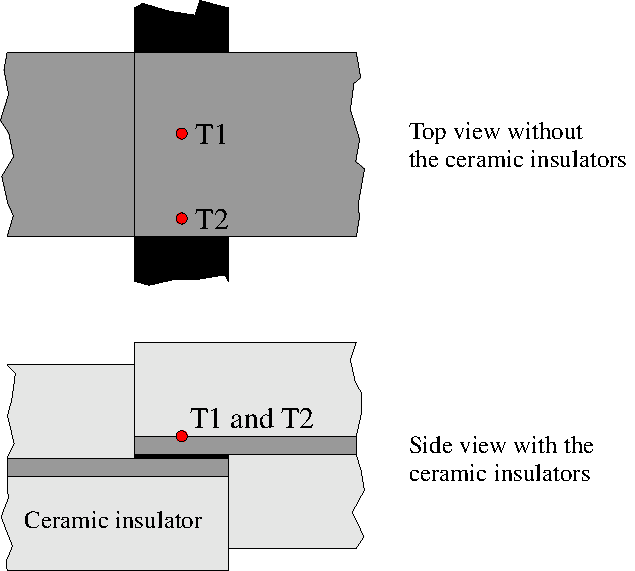
\includegraphics[width=60mm]{thermocouple_welding}
		%\tikzsetnextfilename{thermocouple_welding}
		\usetikzlibrary{arrows.meta,shapes,positioning,shadows,trees,decorations.pathmorphing}

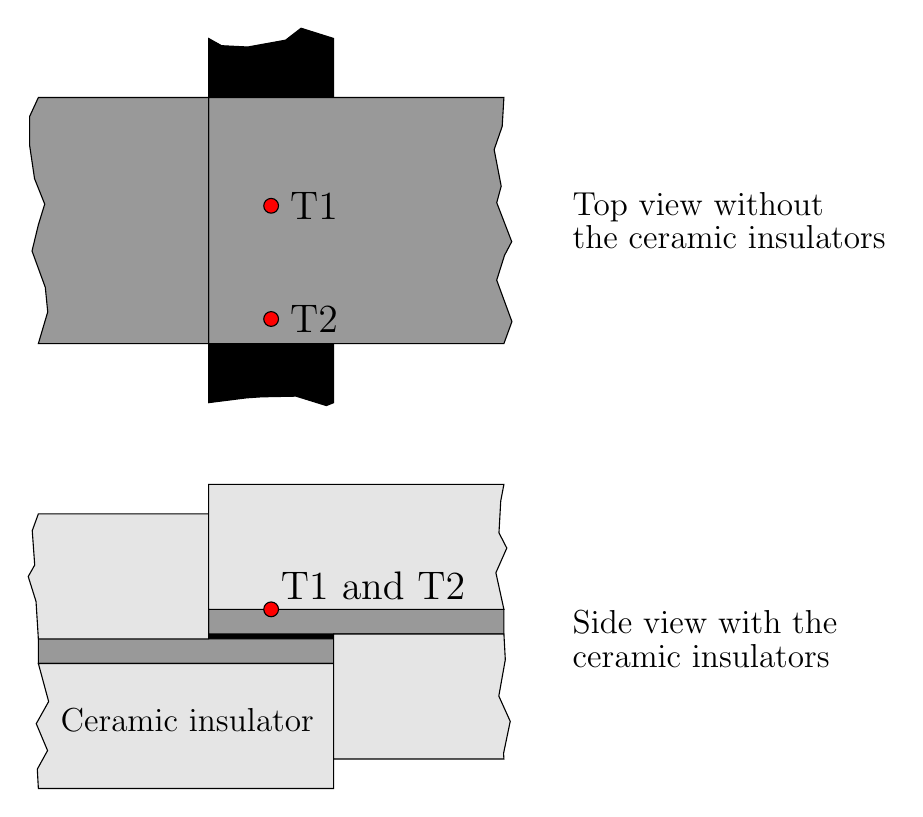
\begin{tikzpicture}[scale=0.125]

%Couleurs
\def \colceramique{black!10}
\def \colcomposite{black!40}

%Définition des dimensions du joint soudé
\def \overlap{12.7}
\def \epceramique{12.7}
\def \epcomposite{2.5}
\def \epnanocomposite{0.5}
\def \longueur{30}
\def \gapfigure{30}
\def \largeursoudure{25}
\def \depassementsoudure{6}
\def \diacercle{0.75}

%%%Vue du dessus %%%
\draw (\longueur+\depassementsoudure,\gapfigure+0.5*\largeursoudure) node [right, align=left]{\large Top view without \\ \large the ceramic insulators};

%Élément chauffant
\draw[black,decoration={random steps, amplitude=4, segment length=10},fill=black] (0,\gapfigure-\depassementsoudure) decorate{-- ++(\overlap,0)} -- ++(0,2*\depassementsoudure+\largeursoudure) decorate{-- ++(-\overlap,0)} -- cycle;

%Adhérent
\draw[black,decoration={random steps, amplitude=4, segment length=10},fill=\colcomposite] 
(0,\gapfigure) -- ++(\longueur,0) decorate{-- ++(0,\largeursoudure)} -- ++(-\longueur,0) -- cycle;
\draw[black,decoration={random steps, amplitude=4, segment length=10},fill=\colcomposite] 
(0,\gapfigure) -- ++(-\longueur+\overlap,0) decorate{-- ++(0,\largeursoudure)} -- ++(\longueur-\overlap,0) -- cycle;

%Position du thermocouple
\draw[fill=red] (0.5*\overlap,\gapfigure+14) circle (0.75) node [right]{\ \Large T1};
\draw[fill=red] (0.5*\overlap,\gapfigure+2.5) circle (0.75) node [right]{\ \Large T2};


%%% Vue du côté %%%
\draw (\longueur+\depassementsoudure,0) node [right, align=left]{\large Side view with the \\ \large ceramic insulators};

%Éléments chauffants
\draw[black,thick,fill=black] (0,0) -- ++(\overlap,0) -- ++(0,\epnanocomposite) -- ++(-\overlap,0) -- cycle;

%Adhérents
\draw[black,decoration={random steps, amplitude=4, segment length=6},fill=\colcomposite] 
(\overlap,0) -- ++(-\longueur,0) decorate{-- ++(0,-\epcomposite)} -- ++(\longueur,0) -- cycle;
\draw[black,decoration={random steps, amplitude=4, segment length=6},fill=\colcomposite] 
(0,\epnanocomposite) -- ++(\longueur,0) decorate{-- ++(0,\epcomposite)} -- ++(-\longueur,0) -- cycle;

%Céramiques
\draw[black,decoration={random steps, amplitude=4, segment length=10},fill=\colceramique] 
(\overlap,-\epcomposite) -- ++(-\longueur,0) decorate{-- ++(0,-\epceramique)} -- ++(\longueur,0) -- cycle;
\draw[black,decoration={random steps, amplitude=4, segment length=10},fill=\colceramique] 
(0,0) -- ++(-\longueur+\overlap,0) decorate{-- ++(0,\epceramique)} -- ++(\longueur-\overlap,0) -- cycle;
\draw[black,decoration={random steps, amplitude=4, segment length=10},fill=\colceramique] 
(\overlap,\epnanocomposite) -- ++(\longueur-\overlap,0) decorate{-- ++(0,-\epceramique)} -- ++(-\longueur+\overlap,0) -- cycle;
\draw[black,decoration={random steps, amplitude=4, segment length=10},fill=\colceramique] 
(0,\epnanocomposite+\epcomposite) -- ++(\longueur,0) decorate{-- ++(0,\epceramique)} -- ++(-\longueur,0) -- cycle;

%Identification des céramiques
\draw (-\longueur+1.1*\overlap,-0.65*\epceramique) node [right, align=left]{ \large Ceramic insulator};

%Position du thermocouple
\draw[fill=red] (0.5*\overlap,\epnanocomposite+\epcomposite) circle (0.75) node [above right]{\Large T1 and T2};


\end{tikzpicture}

		}
		\caption{Location of the thermocouples during the welding process}
		\label{fig:location_thermocouple}
\end{figure} 

\FloatBarrier
%%%%%%%%%%%%%%%%%%%%%%%%%%%%%%%%%%%%%%%%%%%%%%%%%%%%%%%%%%%%%%%%%
							\section{Results and discussion}
%%%%%%%%%%%%%%%%%%%%%%%%%%%%%%%%%%%%%%%%%%%%%%%%%%%%%%%%%%%%%%%%%

%%%%%%%%%%%%%%%%%%%%%%%%%%%%%%%%%%%%%%%%%%%%%%%%%%%%%%%%%%%%%%
\subsection{Simulations results}
%%%%%%%%%%%%%%%%%%%%%%%%%%%%%%%%%%%%%%%%%%%%%%%%%%%%%%%%%%%%%%

\subsubsection{Heat generated by MWCNTs}
	\label{subsection:mechanism1}

\begin{figure}[htb]
	\centering
	\captionsetup{width=125mm}
	\begin{subfigure}{60mm}
		\centering
		\captionsetup{width=75mm}
		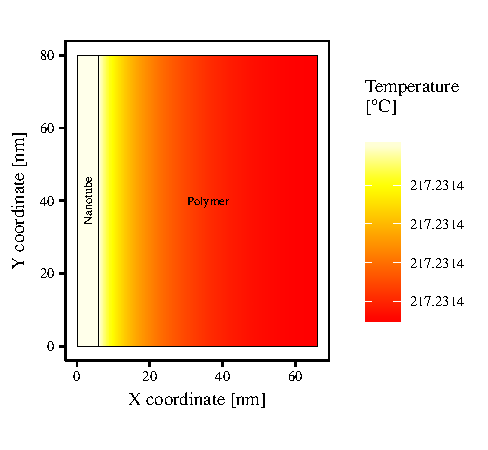
\includegraphics[width=3.25in]{resultats_comsol_axisymetrique_temp}
		\caption{Temperature field}
		\label{fig:temp_axysymmetric}
	\end{subfigure}
	\begin{subfigure}{80mm}
		\centering
		\captionsetup{width=75mm}
		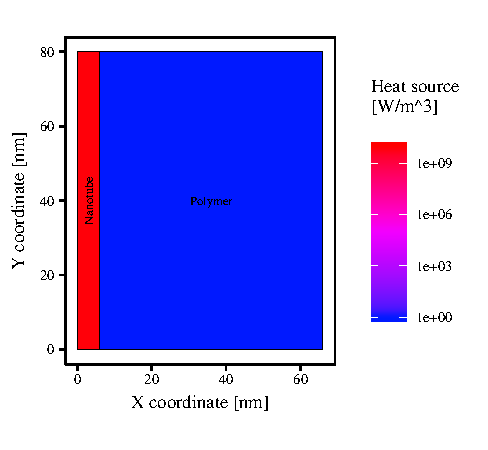
\includegraphics[width=3.25in]{resultats_comsol_axisymetrique_puissance}
		\caption{Heat generation field}
		\label{fig:heat_axysymmetric}
	\end{subfigure}%	
	\caption{Results of the FEM evaluating the heat generation within the MWCNT}
	\label{fig:results_axysymmetric}
\end{figure}

As expected, simulations from the first FEM show resistive heat generated only within the MWCNT (Fig. \ref{fig:heat_axysymmetric}). 
Current went through the conductive MWCNT and thermal conduction heated the polymer. 
A uniform temperature of \SI{217}{\celsius} is obtained for this simulation after \SI{5}{\second} with an electric field of \SI{100}{\volt\per\metre}. 

\subsubsection{Contact resistance heat generation}
	\label{subsection:mechanism2}

\begin{figure}[htb]
	\centering
	\captionsetup{width=125mm}
	\begin{subfigure}{60mm}
		\centering
		\captionsetup{width=75mm}
		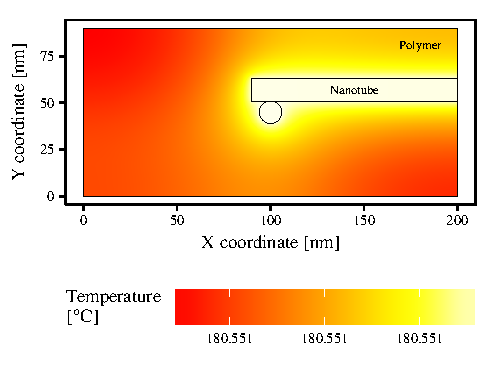
\includegraphics[width=80mm]{resultats_comsol_3D_temp}
		\caption{Temperature field}
		\label{fig:temp_3D}
	\end{subfigure}
	\begin{subfigure}{80mm}
		\centering
		\captionsetup{width=75mm}
		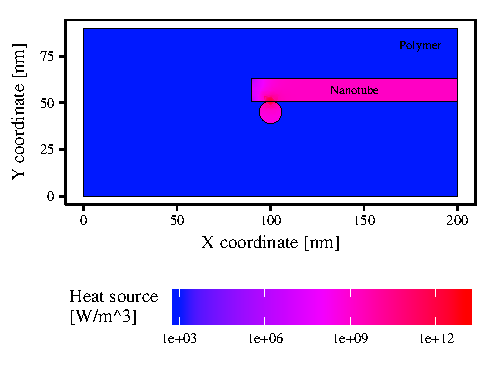
\includegraphics[width=80mm]{resultats_comsol_3D_puissance_log}
		\caption{Heat generation field}
		\label{fig:heat_3D}
	\end{subfigure}
	\caption{Results of the FEM evaluating the effect of charge concentration and contact resistance}
	\label{fig:results_3D}
\end{figure}

For the second FEM, the primary heat source was located at the contact point between the MWCNTs (Fig. \ref{fig:heat_3D}).
Contribution from joule heating within the MWCNTs was also present in the model with a power density 4 orders of magnitude lower.  
A uniform temperature profile is seen in MWCNTs, this is due to their high thermal conductivity. 
A uniform temperature of \SI{141}{\celsius} is obtained for this simulation after \SI{5}{\second} with an electric field of \SI{100}{\volt\per\metre}. 

\subsubsection{Heat generation in the polymer between MWCNTs}
	\label{subsection:mechanism3}

\begin{figure}[htb]
	\centering
	\begin{subfigure}{60mm}
		\centering
		\captionsetup{width=55mm}
		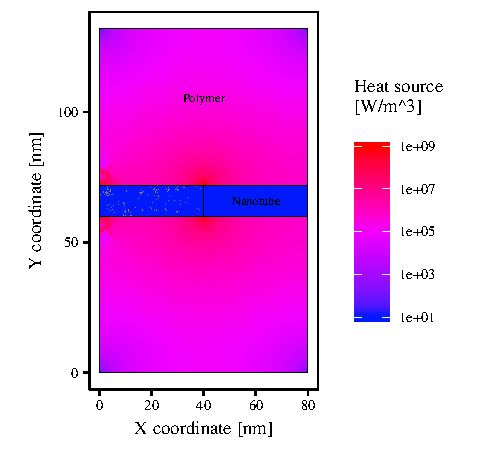
\includegraphics[width=60mm]{resultats_0,1nm_comsol_2D_puissance}
		\caption{\SI{0.1}{\nano\metre} gap, \SI{3.1e9}{\volt\per\metre}}
		\label{fig:result_gap01nm_power}		
	\end{subfigure} 
	\begin{subfigure}{60mm}
		\centering
		\captionsetup{width=55mm}
		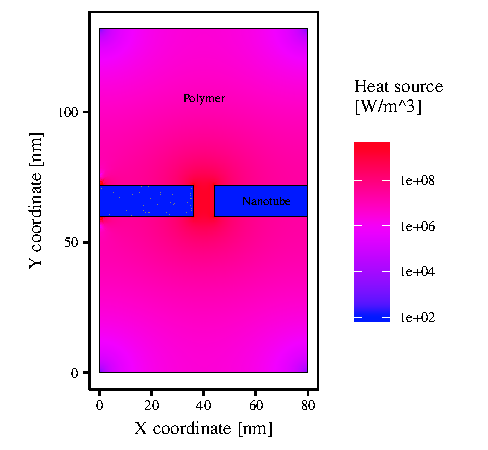
\includegraphics[width=60mm]{resultats_8nm_comsol_2D_puissance}
		\caption{\SI{8}{\nano\metre} gap, \SI{15e9}{\volt\per\metre}}
		\label{fig:result_gap8nm_power}		
	\end{subfigure}
	\caption{Effect of the gap length on the heat generation fields in the case of heat generation within the polymer}
	\label{fig:result_gap_power}
\end{figure}

\begin{figure}[htb]
	\centering
	\begin{subfigure}{60mm}
		\centering
		\captionsetup{width=55mm}
		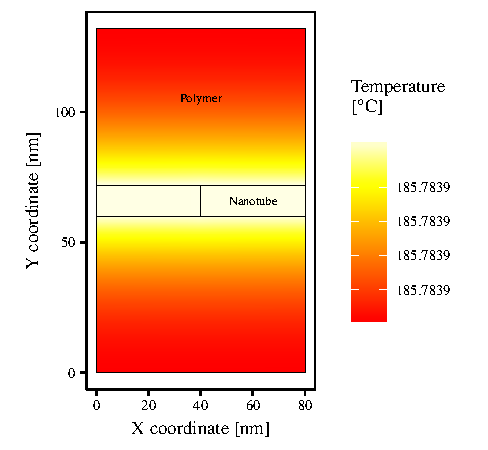
\includegraphics[width=60mm]{resultats_0,1nm_comsol_2D_temp}
		\caption{\SI{0.1}{\nano\metre} gap, \SI{3.1e9}{\volt\per\metre}}
		\label{fig:result_gap01nm_temp}		
	\end{subfigure} 
	\begin{subfigure}{60mm}
		\centering
		\captionsetup{width=55mm}
		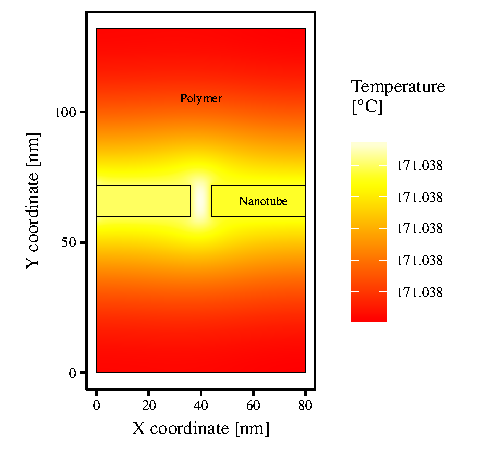
\includegraphics[width=60mm]{resultats_8nm_comsol_2D_temp}
		\caption{\SI{8}{\nano\metre} gap, \SI{15e9}{\volt\per\metre}}
		\label{fig:result_gap8nm_temp}		
	\end{subfigure}
	\caption{Effect of the gap length on the temperature fields in the case of heat generation within the polymer}
	\label{fig:result_gap_temp}
\end{figure}

In the third FEM, heat generation occurred almost exclusively in the polymer matrix (Fig. \ref{fig:result_gap_power}). 
Heat is generated in the bulk of the polymer and a uniform temperature profile is observed in the model (Fig. \ref{fig:result_gap_temp}). 

\FloatBarrier

The third model demonstrate that the electric field required to reach a temperature similar to that of the first 2 models increase sharply when a small gap is introduced in the conductive network (Fig. \ref{fig:result_gap_temp}). 
A gap of \SI{0.1}{\nano\metre}, between adjacent MWCNTs, required a field of \SI{3.1e9}{\volt\per\metre} to produce a temperature field of \SI{170}{\celsius} (Fig. \ref{fig:result_gap01nm_temp}). 
When the gap was increased to \SI{8}{\nano\metre} a field of \SI{15e9}{\volt\per\metre} was necessary (Fig. \ref{fig:result_gap8nm_temp}). 
These electrical field strengths are above the dielectric strength of PEEK (\SI{1.2e9}{\volt\per\metre}) and the current went through the bulk of the polymer matrix. 
That 7 order of magnitude increase in the electrical field, when a gap is introduced, leads to a situation where the third mode of conduction is unlikely to happen in practical applications. 
A connected network of MWCNTs provides pathways of lower resistance for the electrons to flow. 
A sharp increase in the resistance is indicative of a perturbation in the percolated network. 
From these results, it can be concluded that conduction (and thus heat dissipation) within MWCNTs and through their contact points is the main driver for heat generation within a nanocomposite. 
For these mode of conduction, the specific power generated within the REV can be evaluated from the simulations. 
Values of \SI{68}{\watt\per\cubic\centi\metre} and \SI{61}{\watt\per\cubic\centi\metre} were respectively obtained for the first and second models. 

\subsubsection{Timescale analysis}

Although PEEK has poor thermal conductivity, uniform temperature fields with temperature variations not exceeding \SI{1e-5}{\celsius} are observed in the models. 
A comparative numerical analysis of the timescales for thermal diffusion, can explain this behaviour. 
This timescale is evaluated using the time constant for thermal diffusion ($t_D$) : 

\begin{equation}
	t_D = \frac{L^2}{\alpha}
	\label{equa:time_constant}
\end{equation}

\begin{figure}[htb]
	\center
	\captionsetup{width=35mm}
	\resizebox{35mm}{!}{%\\
	%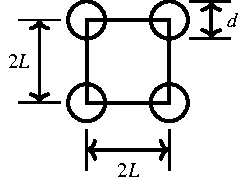
\includegraphics[scale=1]{arrangement_carre}
	%\tikzsetnextfilename{arrangement_carre}
	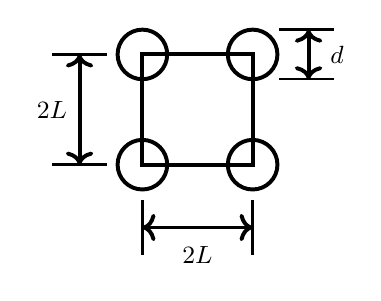
\begin{tikzpicture}[scale=1.4]

\def \l{1}
\def \r{0.225}
\def \vspace{0.32}
\def \lignecote{0.5}

\def \heavy{0.05cm}
\def \light{0.03cm}

\draw[line width=\heavy] (0,0) rectangle (\l,\l);

\draw[line width=\heavy] (0,0) circle (\r);
\draw[line width=\heavy] (\l,0) circle (\r);
\draw[line width=\heavy] (0,\l) circle (\r);
\draw[line width=\heavy] (\l,\l) circle (\r);

\draw[line width=\light] (0,-\vspace) -- + (0,-\lignecote);
\draw[line width=\light] (\l,-\vspace) -- + (0,-\lignecote);
\draw[<->,line width=\heavy] (0,-\vspace-0.5*\lignecote) -- + (\l,0);

\node (A) at (0.5*\l , -\vspace-\lignecote) {\small $2L$};

\draw[line width=\light] (-\vspace,0) -- + (-\lignecote,0);
\draw[line width=\light] (-\vspace,\l) -- + (-\lignecote,0);
\draw[<->,line width=\heavy] (-\vspace-0.5*\lignecote,0) -- + (0,\l);

\node (A) at (-\vspace-\lignecote,0.5*\l ) {\small $2L$};

\draw[line width=\light] (\l+0.75*\vspace,\l-\r) -- + (\lignecote,0);
\draw[line width=\light] (\l+0.75*\vspace,\l+\r) -- + (\lignecote,0);
\draw[<->,line width=\heavy] (\l+\vspace+0.375*\lignecote,\l-\r) -- + (0,2*\r);

\node (A) at (\l+\vspace+0.25*\lignecote+\vspace,\l ) {\small $d$};


\end{tikzpicture}
	}
	\caption{Square packing micromechanic model}
	\label{fig:square_packing}
\end{figure}

Assuming a uniform square packing of evenly distributed particles (Fig. \ref{fig:square_packing}) of known diameter ($d$) and variable volume fractions ($v_f$), it is possible to evaluate the average half distance ($L$) between particles :

\begin{equation}
	L = \sqrt{\frac{\pi \ d^2}{16 \ v_f}}
	\label{equa:L_average}
\end{equation}

The thermal diffusivity ($\alpha$) is defined as a function of thermal conductivity ($k$), density ($\rho$) and specific heat ($C_p$) : 

\begin{equation}
	\alpha = \frac{k}{\rho \ C_p}
	\label{equa:thermal_diffusivity}
\end{equation}

\begin{table}[htb]
\centering
%\resizebox{88mm}{!}{
\begin{tabular}{@{}p{2.4cm}p{2.5cm}p{2cm}p{1.5cm}@{}}
\toprule
Weight fraction of MWCNTs	& Volume fraction of MWCNT	& Average half distance 	& \textbf{Time constant}  		\\ %\midrule
$w_f$								& $v_f$ 							& L 							& $\mathbf{t_D}$            	\\
{[}\%{]}							& {[}\%{]	}						& {[}nm{]} 					& \textbf{{[}s{]}}            	\\ \midrule
1									& 0.65 							& 65.8	 						& $\mathbf{3\times 10^{-8}}$ 	\\ 
5									& 3.31								& 29.2							& $\mathbf{6\times 10^{-9}}$	\\
10									& 6.74								& 20.5							& $\mathbf{3\times 10^{-9}}$	\\
16									& 11.02 							& 16.0 						& $\mathbf{2\times 10^{-9}}$	\\	\bottomrule
\end{tabular}%}
\caption{Timescale for heat conduction}
\label{tab:results_timescale}
\end{table}

Since the thermal conductivity of MWCNTs is very high compared to the polymer, only the properties of the matrix were considered in this timescale analysis. 
Table \ref{tab:results_timescale} presents the time constants calculated for thermal diffusion within the polymer matrix. 
The time constants varied from $3 \times 10^{-8}$ to \SI{2e-9}{\second} for $v_f$ varying from 1\% to 16\%. 
Considering that the simulations looked at Joule heating on a scale closer to the second, the short timescales for thermal diffusion explain the constant temperature fields. 

%%%%%%%%%%%%%%%%%%%%%%%%%%%%%%%%%%%%%%%%%%%%%%%%%%%%%%%%%%%%%%
\subsection{Small scale experiments}
%%%%%%%%%%%%%%%%%%%%%%%%%%%%%%%%%%%%%%%%%%%%%%%%%%%%%%%%%%%%%%

The electrical parameters and maximum surface temperature recorded at steady state are presented in Table \ref{tab:results_lab}. 
From these results, it is possible to calculate the specific electrical power generated within the nanocomposite and evaluate the electrical conductivity. 

\begin{table}[htb]
\centering
%\resizebox{88mm}{!}{
\begin{tabular}{@{}lrrrrr@{}}
\toprule
Voltage 				& Electric							& Current 				& Maximum  					& Specific   										& Nanocomposite's \\ 
 						& field								&  							& surface 					& power   											& electrical \\ 
 						& 										&  							& temperature 				&    													& conductivity \\
{[}\si{\volt}{]} 	& {[}\si{\volt\per\metre}{]} 	& {[}\si{\ampere}{]} 	& {[}\si{\celsius}{]} 	& {[}\si{\watt\per\cubic\centi\metre}{]}	& {[}\si{\siemens\per\centi\metre}{]} \\ \midrule
10 						& 145									& 0.011 					& 24 							& 2		  												& 0.97 \\
20						& 290									& 0.031 					& 30 							& 12	 												& 1.37 \\
30 						& 435									& 0.050 					& 49 							& 28	 												& 1.48 \\
40 						& 580									& 0.073 					& 81 							& 54	 												& 1.59 \\
50 						& 724									& 0.108 					& \textgreater 150 		& 99	 												& 1.89 \\ \bottomrule
\end{tabular}%}
\caption{Electrical results from the small scale experiments}
\label{tab:results_lab}
\end{table}

\begin{figure}[htb]
	\center
	\captionsetup{width=125mm}
	\begin{subfigure}{60mm}
		\center
		\captionsetup{width=60mm}
		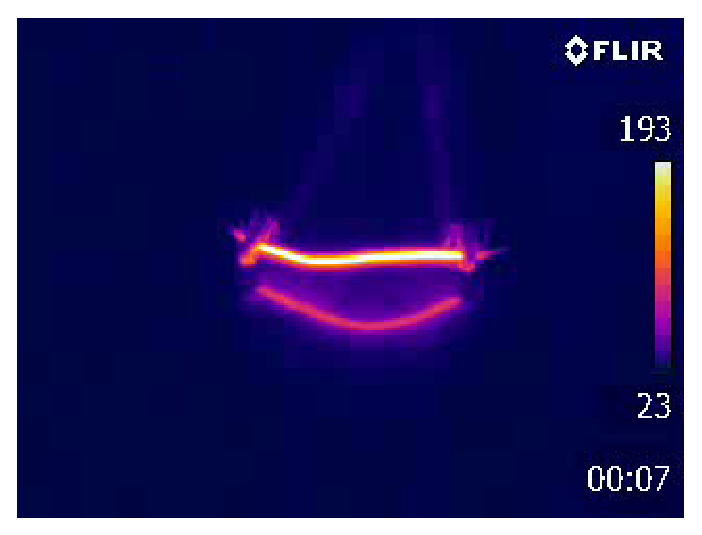
\includegraphics[width=60mm]{output0036}
		\caption{Thermographs in \si{\celsius} of the polymer wire during the small scale experiments under an AC electrical field of \SI{724}{\volt\per\metre}}
		\label{fig:results_thermal}
	\end{subfigure}
	\begin{subfigure}{80mm}
		\center
		\captionsetup{width=78mm}
		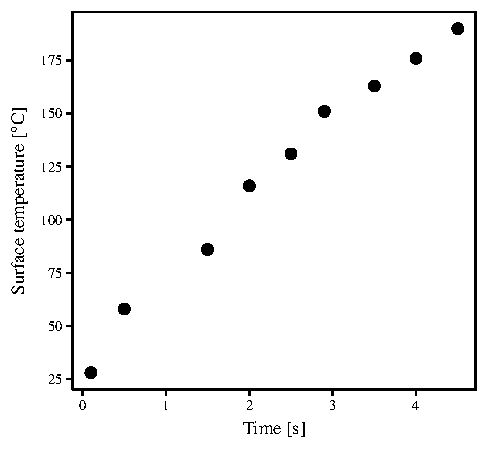
\includegraphics[width=3.25in]{temperature_over_time.pdf}
		\caption{Evolution of the temperature during the small scale experiments under an AC electrical field of \SI{724}{\volt\per\metre}}
		\label{fig:temp_over_time}
	\end{subfigure}%	
	\caption{Temperature of the wire during the experiment}
	\label{fig:results_lab}
\end{figure}

As expected, an increase of the electric field produces higher surface temperatures with higher currents flowing through the sample. 
Under an electric field of \SI{700}{\volt\per\metre}, the wire reached a surface temperature of \SI{190}{\celsius} after 5 seconds (Fig. \ref{fig:results_thermal}), corresponding to a heating rate of \SI{33}{\celsius\per\second} (Fig. \ref{fig:temp_over_time}). 
Although a higher electrical field was required (\SI{700}{\volt\per\metre} vs \SI{100}{\volt\per\metre}), the small scale experiments produced uniform heating at the surface of the nanocomposite wire. 
It is also possible to verify, from the heating rate ($\dot{T}$) (in \si{\celsius}) and the material properties (Tab. \ref{tab:material_properties}), that the specific thermal power (in \si{\watt\per\cubic\metre}) dissipated by the nanocomposite is in agreement to the specific electrical power measured (Eq. \ref{eq:specific_power}). 

\begin{equation}
P_{specific} = \rho \ C_p \ \dot{T}
\label{eq:specific_power}
\end{equation}

Using the mixing rule, the density is estimated at \SI{1410}{\kilo\gram\per\cubic\metre} and the specific heat at \SI{1730}{\joule\per\kilo\gram\per\celsius}. 
This results in a specific thermal power of \SI{80}{\watt\per\cubic\centi\metre} that is similar to the specific electrical powers in Tab. \ref{tab:results_lab}. 
The uniform heating observed in addition to the ability to tune the power output are important characteristics for the resistance welding process.  

\FloatBarrier

%%%%%%%%%%%%%%%%%%%%%%%%%%%%%%%%%%%%%%%%%%%%%%%%%%%%%%%%%%%%%%
\subsection{Welding experiments}
%%%%%%%%%%%%%%%%%%%%%%%%%%%%%%%%%%%%%%%%%%%%%%%%%%%%%%%%%%%%%%

\subsubsection{Nanocomposite heating elements}

A nanocomposite with 16\% weight fraction of MWCNTs and a matrix composed of PEEK was produced for the small scale experiments. 
PEEK was initially chosen for its high melting temperature and thermal stability. 
The transition to a PEI matrix, for the welding experiments, lowers the welding temperatures and the energy requirements. 
The electrical conductivity of nanocomposites with 5\%, 10\% and 15\% mass fractions of MWCNTs was measured at respectively of 0.27, 0.79 and \SI{0.92}{\siemens\per\centi\metre} with standard deviations of 0.08, 0.06 and \SI{0.30}{\siemens\per\centi\metre}. 
It was decided that the marginal gain in conductivity between 10\% and 15\% mass fraction of MWCNTs was not worth the increased cost and production problems associated with high particle loading. 
PEI nanocomposite films with 10\% mass fraction of MWCNTs were used as heating elements during the welding tests. 
The electrical resistance between the copper electrodes was \SI{50}{\ohm} at a contact pressure of \SI{2.4}{\mega\pascal}. 

\subsubsection{Constant voltage welding}

Like in traditional resistance welding, initial welding experiments were performed under constant voltage. 
Normal small variations in the electrical conductivity of the nanocomposite were negatively affecting the reproducibility of the process. 
One samples showed signs of welding while others, under similar conditions, would give unpredictable results. 
This mode of operation caused to much variation between samples to be considered adequate and switching to operation under constant power solved these problems. 
\todo[inline, color=green!40]{I don't think that a picture of failed welds is pertinent in this section but I do have some that could be added if needed}

\subsubsection{Constant power welding}
\FloatBarrier

\missingfigure{Photo of fractography 350kW-90-10-150-3UD}


\todo[inline]{The section describing the results under constant power}


\begin{figure}[h]
	\center
	\captionsetup{width=78mm}
	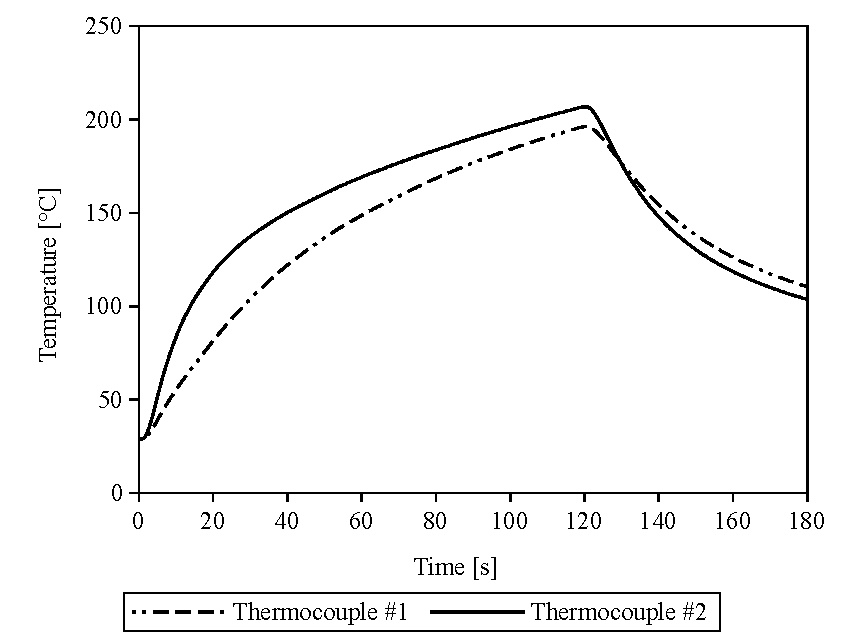
\includegraphics[width=3.25in]{temp_welding_350kw.pdf}
	\caption{Evolution of the temperature during the welding process at \SI{350}{\kilo\watt\per\square\metre}}
	\label{fig:temp_350kW_120_10_150_3UD}
\end{figure}




\begin{table}[htb]
\centering
\resizebox{\textwidth}{!}{
\pgfplotstabletypeset[header=false,
							col sep=comma,
							every head row/.style={
									before row={\toprule
									Power density & Electrode distance & Pressure & Values & \multicolumn{4}{c}{Time} \\
									$[$\si{\kilo\watt\per\square\metre}$]$ & [\si{\milli\metre}] & [\si{\mega\pascal}] & & \multicolumn{4}{c}{[\si{\second}]} \\ },
									output empty row
														},
							every last row/.style={
														after row=\bottomrule
														},
							every row no 0/.style={
														after row=\midrule
														},
							display columns/3/.style={
													string type
													}
							]{resultats_SLS.csv}}

\caption{Results of SLS tests and fractography analysis}
\label{tab:SLS_and_fractography_results}
\end{table}


\FloatBarrier

\todo[inline, color=green!40]{I don't think that I will need to include the FTIR results}

\todo[inline]{Discussion of the results, their limits and links to the results of the other tests}

%%%%%%%%%%%%%%%%%%%%%%%%%%%%%%%%%%%%%%%%%%%%%%%%%%%%%%%%%%%%%%%%%
							\section{Conclusion}
%%%%%%%%%%%%%%%%%%%%%%%%%%%%%%%%%%%%%%%%%%%%%%%%%%%%%%%%%%%%%%%%%



%%%%%%%%%%%%%%%%%%%%%%%%%%%%%%%%%%%%%%%%%%%%%%%%%%%%%%%%%%%%%%%%%
							\section{Acknowledgements}
%%%%%%%%%%%%%%%%%%%%%%%%%%%%%%%%%%%%%%%%%%%%%%%%%%%%%%%%%%%%%%%%%

This work was supported by Airbus Safran Launcher and CREPEC. 
The authors also thank Prof. G.S. Patience for the use of the thermal imaging camera and Prof D. Therriault for access to the microcompounder. 

%%%%%%%%%%%%%%%%%%%%%%%%%%%%%%%%%%%%%%%%%%%%%%%%%%%%%%%%%%%%%%%%%
							\section*{References}
%%%%%%%%%%%%%%%%%%%%%%%%%%%%%%%%%%%%%%%%%%%%%%%%%%%%%%%%%%%%%%%%%

\bibliographystyle{model4-names}
\bibliography{Article_soudage_nano_1}
%\pagebreak

%\section{Figures}
%\FloatBarrier

\end{document}
